\chapter{Theoretical Foundations}\label{ch:theory}
\section{Detection as the engineering model}
For a canonical RGB image $I$ of width $W$ and height $H$, a detector with
parameters $\theta$ produces a finite set
\begin{equation}
 D_\theta(I)=\{(b_i,c_i,s_i)\}_{i=1}^{n},
 \qquad b_i=(x_{1i},y_{1i},x_{2i},y_{2i}).
\end{equation}
Here $c_i$ belongs to the selected model's task namespace and $s_i$ is a model
confidence. Box corners are measured in original-image pixels with positive
width and height. The confidence is not assumed to be a calibrated probability
of a dangerous device. A task map is needed to interpret labels; a model output
index and a dataset category ID are different identifiers.

\begin{figure}[htbp]
\centering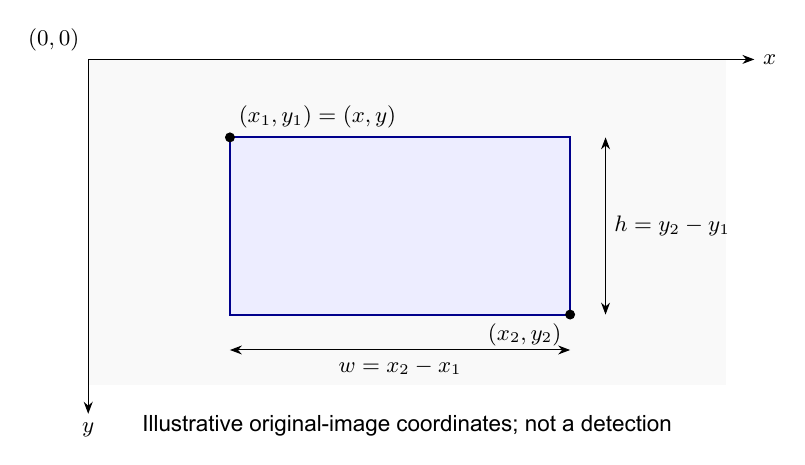
\includegraphics[width=0.82\textwidth]{coordinates.png}
\caption{Original explanatory diagram of corner and COCO box coordinates.
The rectangle is illustrative and is not a scan or model prediction.}
\label{fig:coordinates}
\end{figure}

COCO annotations use $(x,y,w,h)$. Conversion to original-pixel corners is
\begin{equation}
 (x_1,y_1,x_2,y_2)=(x,y,x+w,y+h),
\end{equation}
with inverse $(x_1,y_1,x_2-x_1,y_2-y_1)$. Any resizing or letterboxing inside the
backend must be reversed before the shared contract is emitted. The software
does not repair malformed source geometry silently. Figure~\ref{fig:coordinates}
fixes the convention used in this report.

\section{Localization and detection metrics}
For predicted region $B_p$ and reference region $B_g$, intersection over union is
\begin{equation}
 \operatorname{IoU}(B_p,B_g)=\frac{|B_p\cap B_g|}{|B_p\cup B_g|}.
\end{equation}
At a declared score threshold and matching rule, precision and recall are
\begin{equation}
 P=\frac{TP}{TP+FP},\qquad R=\frac{TP}{TP+FN}.
\end{equation}
Their denominators and undefined cases need explicit treatment. A missed
annotated threat contributes a false negative under the frozen matching rule;
an unannotated detection is not automatically a physical false alarm because
annotation completeness may itself be limited.

COCO AP@[.50:.95] summarizes detection over IoU thresholds from 0.50 to 0.95;
AP50 reports the 0.50 case, and AR summarizes recall under the evaluator's
detection limits. These definitions are implemented by the official evaluator
and must be interpreted with its settings and task maps~\citep{lin2014coco}.
The validation objective returns AP as a fraction from 0 to 1. Published tables
may display percentages; comparing them requires an explicit scale conversion.

\section{Training and validation independence}
Let $T$ be the published training image set and $E$ the published test set.
Controlled improvement requires disjoint fit and validation partitions
$T_f,T_v\subset T$ such that $T_f\cap T_v=\varnothing$ and
$T_f\cup T_v=T$, subject to the reviewed data policy. Exact duplicate bytes and
verified physical groups must not cross $T_f$ and $T_v$. A connected group may
contain several images, so a target 80/20 fraction need not be attained exactly.

The author checkpoints may have seen all published training images. Carving
validation from those images does not make them unseen for those checkpoints.
For controlled U/T experiments, both models start from general pretraining
with documented exclusion evidence and the same task-head initialization
procedure. They share the fixed partition and comparable training budget;
the tuned model's choices are selected on validation, not on the test set.

\section{Optimization and experiment identity}
The planned search objective is
\begin{equation}
 \lambda^*=\arg\max_{\lambda\in\Lambda}
 \operatorname{AP}(f_{\theta(T_f,\lambda)},T_v),
\end{equation}
where $\lambda$ denotes the declared hyperparameters. Optuna supports trial
search and pruning~\citep{akiba2019optuna}; this does not establish that an
improvement exists. Untuned and tuned inference records use distinct output
checkpoint hashes with a common starting-weight parent hash. Matching that
parent is necessary but insufficient: code, task, partition, settings, seeds
and training budgets also need review.

\section{Limits of the model}
Single-image box detection represents appearance and location. It does not
establish chemical composition, electrical connectivity or assembly intent.
FALCON's compositional formulation motivates asking about relationships, but
does not remove the need for suitable supervision and case evaluation
\citep{michael2026falcon}. RayGuard's P2 interface therefore requires external
case provenance and keeps missing scans visible. No mathematical aggregation
rule is presented here as an implemented distributed detector.
